\documentclass[9pt,aspectratio=169]{beamer}
\usetheme{VK}

\usepackage{dsfont}
\usepackage{bm}
\usepackage{xunicode}
\usepackage{xltxtra}
\usepackage{xecyr}
\usepackage{inputenc}

\usepackage{pdfpages}
\usepackage{longtable}
\usepackage{multicol}

\usepackage{tikz}
\usetikzlibrary{angles,quotes}

\usepackage{mwe}
\usepackage{multirow}

\usepackage{csquotes}

\usepackage[style=verbose-ibid,backend=bibtex]{biblatex}
\addbibresource{references.bib}

\date[]{}
\title[]{Soluzione di Fully Fuzzy Linear Systems}
\author[]{Gambuti Giovanni Pasquale}

\AtEndDocument{\usebeamertemplate{endpage}}

\begin{document}
\maketitle
\begin{frame}{Problema:}
    "Linear system of equations are vital for contemplating and comprehending an expansive extent of the issues in connected science, ordinarily in numerous applications a portion of the parameters in our issues are spoken to fuzzy numbers; presented the ideas of fuzzy numbers and fuzzy math, fuzzy numbers number-crunching is connected and valuable in calculation of direct frameworks." \\
    
    \hfill\break
    estratto da: \cite{eliminazione}

\end{frame}
\begin{frame}{Cos'e' la logica Fuzzy?}
\begin{multicols}{2}
La \textbf{logica fuzzy} (o logica sfumata) e' una logica in cui si puo' attribuire a ciascuna proposizione un grado di verita' diverso da 0 e 1 e compreso tra di loro. E' una logica polivalente, ossia un'estensione della logica booleana. E' legata alla teoria degli insiemi sfocati. \\Con grado di verita' o valore di appartenenza si intende quanto e' vera una proprieta', che puo' essere, oltre che vera (= a valore 1) o falsa (= a valore 0) come nella logica classica, anche parzialmente vera e parzialmente falsa.

\begin{figure}[h]
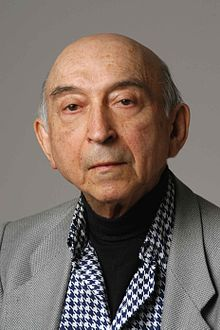
\includegraphics[width=0.33\textwidth]{images/Lotfi_Zadeh_Berkeley_c.jpg}
\caption{Lotfi Aliasker Zadeh, fondatore della logica Fuzzy}
\end{figure}
    
\end{multicols}

\end{frame}

\begin{frame}{Logica Fuzzy}
Nella logica classica, un caso puo' avere due valori, \textit{Vero o Falso};\\ Nella logica fuzzy invece i valori possono essere \textbf{Vero, Falso oppure un valore intermedio tra i due}.\\
I connettivi che si usano nella logica fuzzy sono i seguenti:
\begin{itemize}
    \item $\text{AND}  \ \wedge$
    \item $\text{OR} \ \vee$
    \item $\text{NOT} \ \neg$
    \item $\text{IF-THEN} \ \Rightarrow$
    \item $\text{IF-AND-ONLY-IF} \ \Leftrightarrow$
\end{itemize}
\end{frame}

\begin{frame}{Connettivi logica Fuzzy}
Il risultato dei connettivi logici Fuzzy e' descritto dalle tabelle di verita':\\

\begin{longtable}{cc|c|c|c|c}
p & q & p AND q & p OR q & p IF-THEN q & p IF-AND-ONLY-IF q \\ \hline
\endfirsthead
%
\endhead
%
0 & 0 & 0       & 0      & 0           & 0                  \\
0 & 1 & 1       & 0      & 1           & 1                  \\
1 & 0 & 1       & 0      & 0           & 1                  \\
1 & 1 & 1       & 1      & 0           & 0                 
\end{longtable}
\end{frame}

\section{Definizioni}
\begin{frame}{Numeri Fuzzy} Un numero fuzzy e' la generalizzazione di un numero reale, nel senso che non riferisce un preciso valore ma un range di possibili valori. un qualsiasi numero fuzzy, $\tilde{A}$ = (p, q, r), ha determinate proprieta' e operazioni possibili.\\
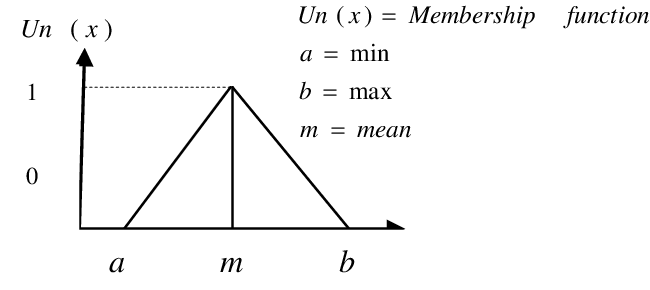
\includegraphics[scale=0.5]{images/Triangular-fuzzy-number-diagram.png}


%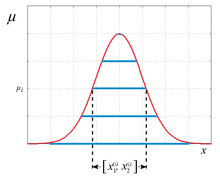
\includegraphics[scale=0.5]{images/220px-Fuzzy_arithmetic.png}
\end{frame}

\begin{frame}{Operazioni aritmetiche sui numeri Fuzzy triang.}

\ddef{Oper. aritmetiche}{
        \begin{equation}
        \begin{aligned}
    \text{considerando due numeri Fuzzy triangolari }\tilde{A}=(p,q,r) \text{ e } \tilde{B}=(s,m,n). \\
\text{Addizione: } \tilde{A} \oplus \tilde{B} = (p,q,r)\oplus(s,m,n)=(p+s,q+m,r+n).\\
\text{Sottrazione: } \tilde{A}\ominus\tilde{B}=(p,q,r) \ominus(s,m,n)=(p-s,q-m,r-n).\\
\text{Moltiplicazione: }\tilde{A}\otimes \tilde{B}=(p,q,r)\otimes(s,m,n)=(ps,pm+sq,pm+sr).\\
\text{Molt. per uno scalare: } \lambda \otimes \tilde{A} =\lambda \otimes(p,q,r)= 
\begin{cases} 
(\lambda p, \lambda q, \lambda r) \ se \ \lambda\ge 0 \\
(-\lambda p, -\lambda q, -\lambda r) \ se \ \lambda \textless  0
\end{cases}
        \end{aligned}
\end{equation}
    }
\end{frame}

\begin{frame}{Sistemi lineari e FFLS}
Le equazioni lineari vengono utilizzate per descrivere molte tra le relazioni e progressi nel mondo reale, come ad esempio:
\begin{itemize}
    \item predire profitti (e altre applicazioni in economia)
    \item calcolare la velocita' di una reazione, in chimica
    \item molti problemi di Fisica, come ad esempio il moto di un proiettile
    \item ecc.
\end{itemize}
    In particolare, \textit{un sistema lineare dove gli elementi della matrice dei coefficienti e quelli del vettore dei termini noti sono numeri fuzzi, si definisce Fully Fuzzy Linear System (FFLS)}
\end{frame}

\begin{frame}{Metodi di risoluzione}
    Per risolvere il sistema abbiamo due metodi:
    \begin{itemize}
        \item Utilizzando l'eliminazione di Gauss Jordan, dopo aver ridotto il sistema in matrici.\\ \cite{eliminazione}
        \item utilizzando il metodo della ST Decompopsition. \\ \cite{STdecomp}
    \end{itemize} 
    
    noi utilizzeremo il primo metodo, dato che lo conosciamo gia' dalle precedenti lezioni, applicato ai sistemi di equazioni lineari.\\
    \textbf{$\rightarrow$ Esaminiamo meglio il metodo con un esempio:}
\end{frame}

\begin{frame}{}
   % 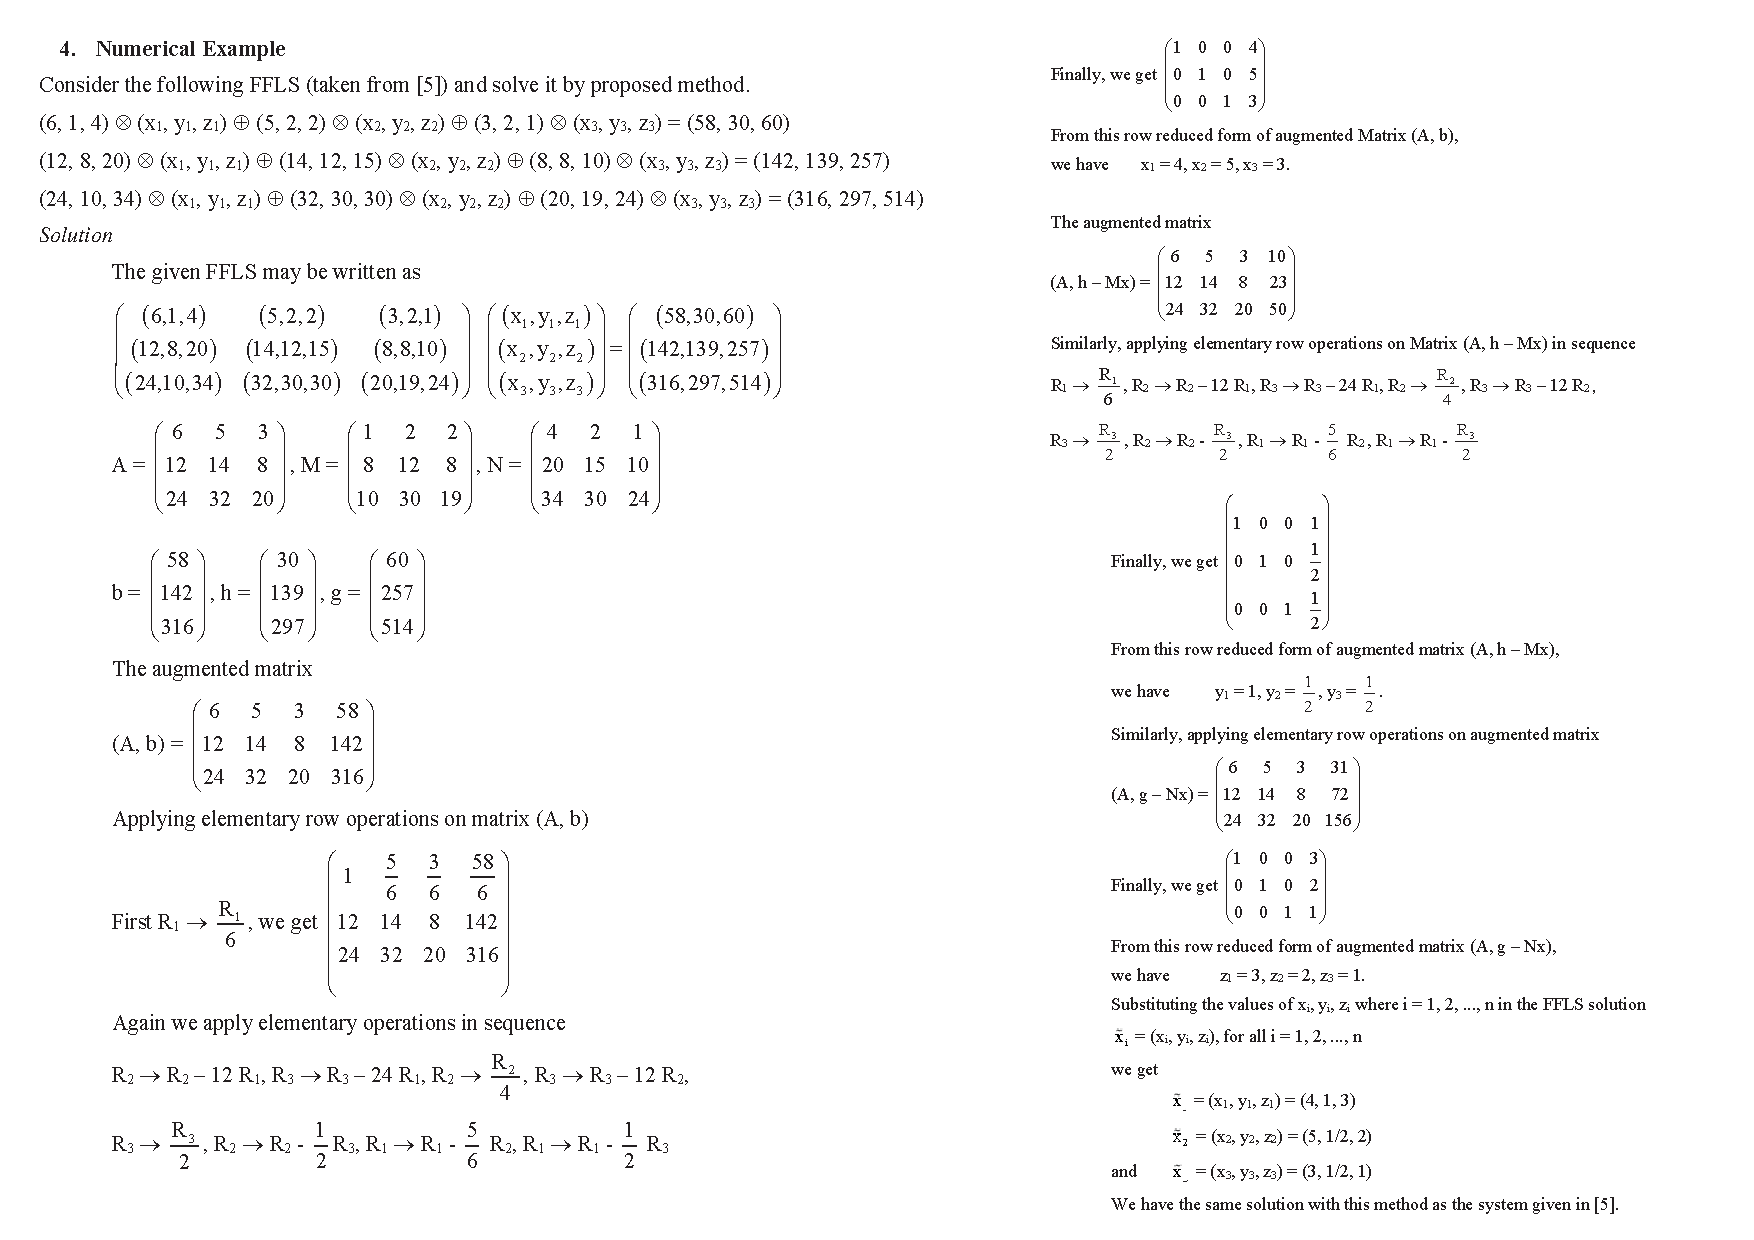
\includepdf[]{images/gaussjordan-fuzzy.pdf}
    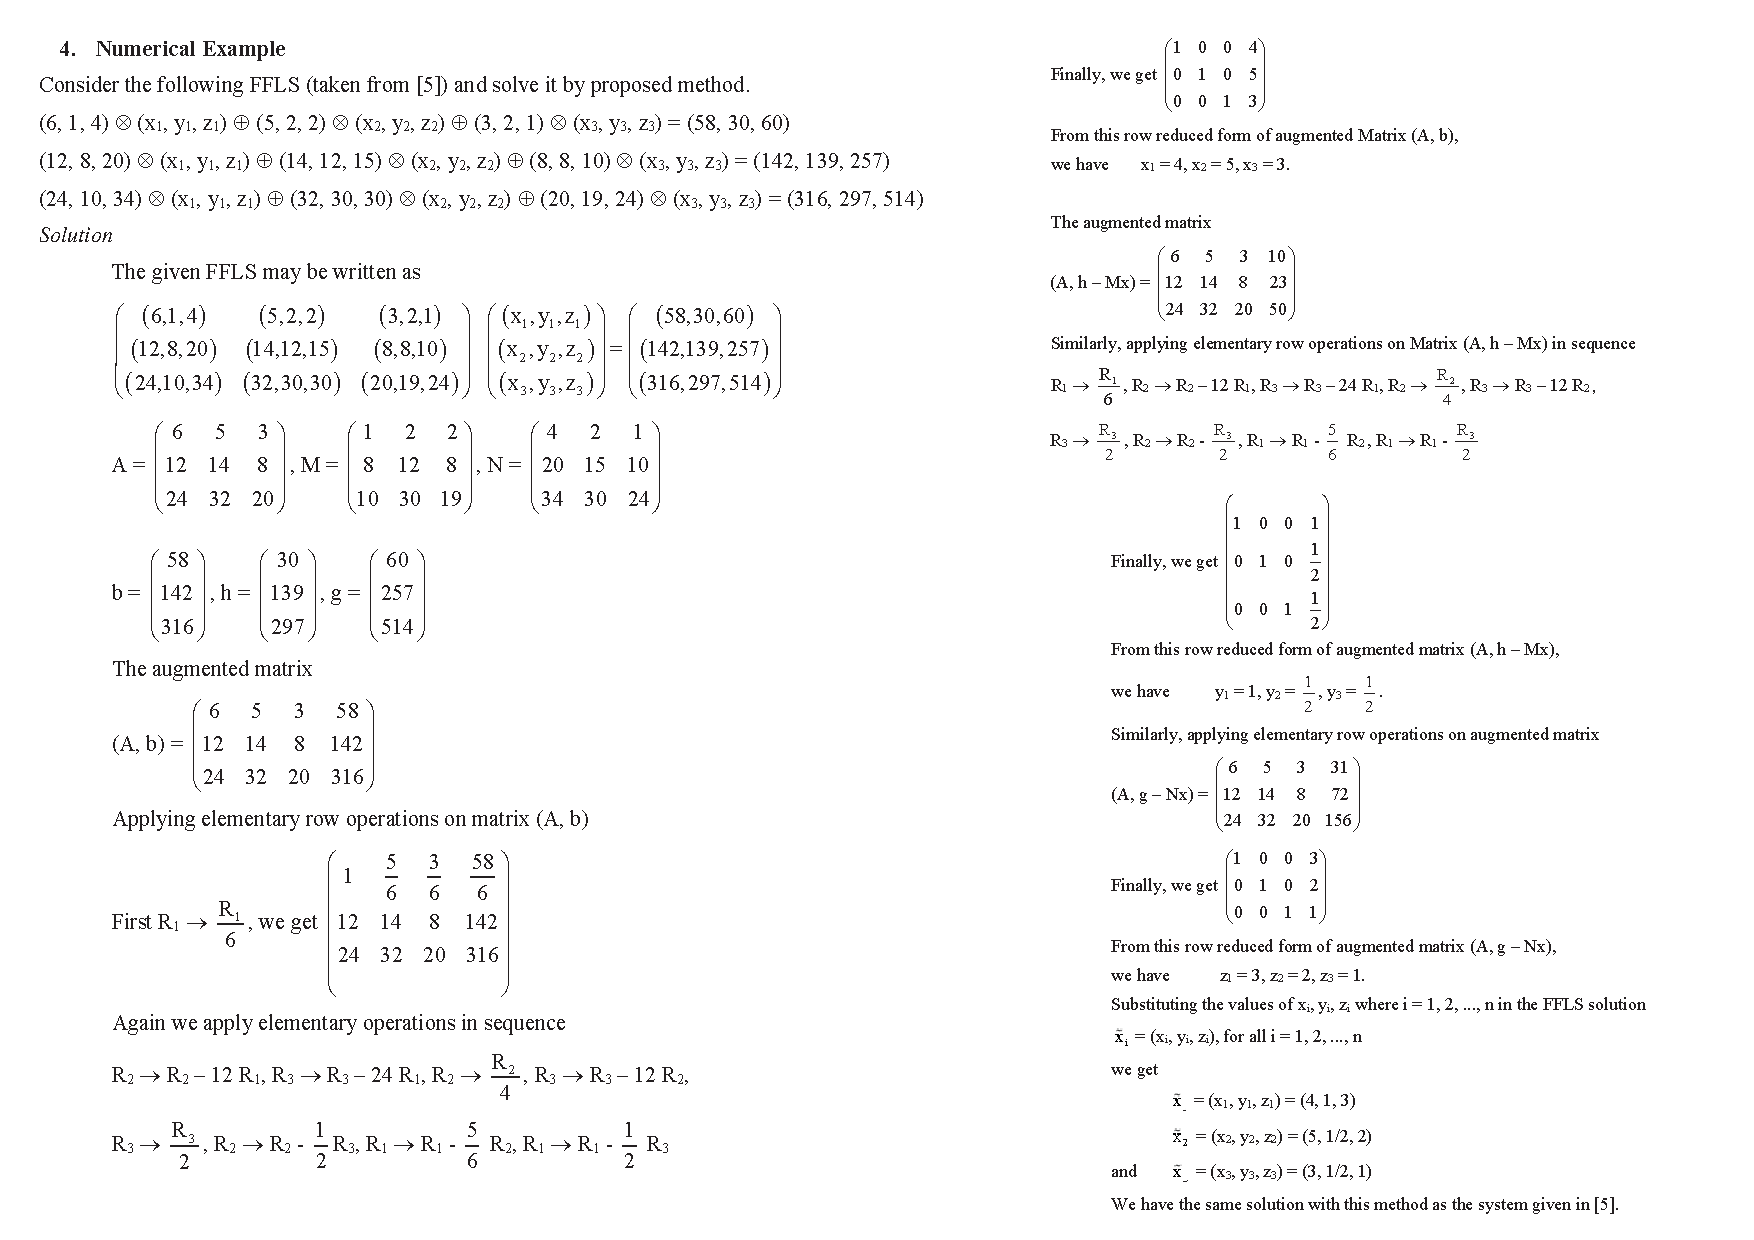
\includegraphics[scale=0.4]{images/gaussjordan-fuzzy.pdf}
\end{frame}


\end{document} 